%%%%%%%%%%%%%%%%%%%%%%%%%%%%%%%%%%%%%%%%%
% Structured General Purpose Assignment
% LaTeX Template
%
% This template has been downloaded from:
% http://www.latextemplates.com
%
% Original author:
% Ted Pavlic (http://www.tedpavlic.com)
%
% Note:
% The \lipsum[#] commands throughout this template generate dummy text
% to fill the template out. These commands should all be removed when 
% writing assignment content.mus
%
%%%%%%%%%%%%%%%%%%%%%%%%%%%%%%%%%%%%%%%%%

%----------------------------------------------------------------------------------------
%	PACKAGES AND OTHER DOCUMENT CONFIGURATIONS
%----------------------------------------------------------------------------------------

\documentclass{article}

%\usepackage[brazilian]{babel}
\usepackage[utf8]{inputenc}
\usepackage{fancyhdr} % Required for custom headers
\usepackage{lastpage} % Required to determine the last page for the footer
\usepackage{extramarks} % Required for headers and footers
\usepackage{graphicx} % Required to insert images
\usepackage{float}
\usepackage{listings}
\usepackage[fleqn]{amsmath}
\usepackage{amsthm}
\usepackage[colorlinks=true, pdfborder={0 0 0}, urlcolor=blue, linkcolor=black]{hyperref}
\usepackage{natbib}
\usepackage{tikz}

\usepackage{algorithm}% http://ctan.org/pkg/algorithms
\usepackage{algpseudocode}% http://ctan.org/pkg/algorithmicx
\usepackage{algorithmicx}

\graphicspath{ {img/} }

\renewcommand{\.}{. \;}
\theoremstyle{definition}
\newtheorem*{definition}{Definition}
\newtheorem*{example}{Example}

\theoremstyle{plain}
\newtheorem{theorem}{Theorem}

\theoremstyle{remark}
\newtheorem*{remark}{Remark}

\newcommand{\pto}{\nrightarrow}
\newcommand{\ptree}[3]{
	\ifx&#2&%
	(#1 \rightrightarrows #3)
	\else
	(#1^#2 \rightrightarrows #3)
	\fi
}

\newcommand{\allgraphs}[1]{\mathcal{G}_{#1}}
\newcommand{\alltgraphs}[1]{\mathcal{TG}_{#1}}
\newcommand{\emptyGraph}{\varepsilon}
\newcommand{\startG}[1]{Z_{#1}}
\newcommand{\startTG}[1]{Z_{#1}}
\newcommand{\pro}{\to}

\newcommand{\rel}{\sim}
\newcommand{\rrestr}{\triangleright}

\newcommand{\source}{\operatorname{s}}
\newcommand{\Source}{\operatorname{S}}
\newcommand{\target}{\operatorname{t}}
\newcommand{\Target}{\operatorname{T}}


\newcommand{\neigh}[1]{\operatorname{neigh}_{#1}}
\newcommand{\scont}[2]{\eta_{#1}(#2)}
\newcommand{\cont}[2]{\operatorname{cont}_{#1}(#2)}
\newcommand{\emb}[1]{\operatorname{emb}(#1)}

\newcommand{\st}{\; | \;}
\newcommand{\isomorph}{\cong}
\newcommand{\ms}[1]{\overset{#1}{\leftarrow}}
\newcommand{\mt}[1]{\overset{#1}{\rightarrow}}
\newcommand{\cderiv}[3]{
	\ifx&#2&%
	\overset{#1}{\Rrightarrow}_{#3}
	\else
	\overset{#1,#2}{\Rrightarrow}_{#3}
	\fi
}
\newcommand{\deriv}[3]{
	\ifx&#2&%
	\overset{#1}{\Rightarrow}_{#3}
	\else
	\overset{#1,#2}{\Rightarrow}_{#3}
	\fi
}
\newcommand{\derivtr}[3]{
	\ifx&#2&%
	\overset{#1}{\Rightarrow^*}_{#3}
	\else
	\overset{#1,#2}{\Rightarrow^*}_{#3}
	\fi
}
\newcommand{\tcderiv}[3]{
	\ifx&#2&%
	\overset{#1}{\Rrightarrow}_{#3}
	\else
	\overset{#1,#2}{\Rrightarrow}_{#3}
	\fi
}
\newcommand{\tderiv}[3]{
	\ifx&#2&%
	\overset{#1}{\Rightarrow}_{#3}
	\else
	\overset{#1,#2}{\Rightarrow}_{#3}
	\fi
}
\newcommand{\tderivtr}[3]{
	\ifx&#2&%
	\overset{#1}{\Rightarrow^*}_{#3}
	\else
	\overset{#1,#2}{\Rightarrow^*}_{#3}
	\fi
}

\newcommand{\?}{\operatorname{\textbf{?}}}
\renewcommand{\:}{\operatorname{\textbf{:}}}
\newcommand{\Break}{\textbf{break}}

\tikzstyle{grammar}=[shorten >=1pt,->,draw=black!50]
\tikzstyle{graph}=[shorten >=1pt,->,draw=black!50]
\tikzstyle{rid} = [align=left, anchor=east]
\tikzstyle{nont}=[rectangle,inner sep=5pt, draw, fill=white, minimum width=20pt]
\tikzstyle{t}=[circle,inner sep=3pt, draw, fill=white, minimum width=15pt]
\tikzstyle{g}=[inner sep=3pt, fill=white]
\tikzstyle{lhs}=[inner sep=5pt, fill=white]
\tikzstyle{w}=[circle, inner sep=2pt, below=8pt, draw, fill=white]
\tikzstyle{edge}=[->, very thick, -latex]
\tikzstyle{edgeLabel}=[midway, above]
\tikzstyle{wedge}=[-, thick]
\tikzstyle{biedge}=[-, very thick]
\tikzstyle{pipe}=[-, very thick]
\tikzstyle{morph}=[-, very thick, dashed, -latex]


% Margins
\topmargin=-0.45in
\evensidemargin=0in
\oddsidemargin=0in
\textwidth=6.5in
\textheight=9.0in
\headsep=0.25in 

\linespread{1.1} % Line spacing

% Set up the header and footer
\pagestyle{fancy}
\lhead{\hmwkAuthorName} % Top left header
%\chead{\hmwkClass\ (\hmwkClassInstructor\ \hmwkClassTime): \hmwkTitle} % Top center header
\rhead{\hmwkClass: \hmwkTitle} % Top center header
%\rhead{\firstxmark} % Top right header
\lfoot{\lastxmark} % Bottom left footer
\cfoot{} % Bottom center footer
\rfoot{Page\ \thepage\ of\ \pageref{LastPage}} % Bottom right footer
\renewcommand\headrulewidth{0.4pt} % Size of the header rule
\renewcommand\footrulewidth{0.4pt} % Size of the footer rule

\setlength\parindent{0pt} % Removes all indentation from paragraphs

%----------------------------------------------------------------------------------------
%	DOCUMENT STRUCTURE COMMANDS
%	Skip this unless you know what you're doing
%----------------------------------------------------------------------------------------

% Header and footer for when a page split occurs within a problem environment
\newcommand{\enterProblemHeader}[1]{
\nobreak\extramarks{#1}{#1 continues in next page\ldots}\nobreak
\nobreak\extramarks{#1 (continuation)}{#1 continues in next page\ldots}\nobreak
}

% Header and footer for when a page split occurs between problem environments
\newcommand{\exitProblemHeader}[1]{
\nobreak\extramarks{#1 (continuation)}{#1 continues in next page\ldots}\nobreak
\nobreak\extramarks{#1}{}\nobreak
}

\setcounter{secnumdepth}{0} % Removes default section numbers
\newcounter{homeworkProblemCounter} % Creates a counter to keep track of the number of problems

\newcommand{\homeworkProblemName}{}
\newenvironment{homeworkProblem}[1][\arabic{homeworkProblemCounter}]{ % Makes a new environment called homeworkProblem which takes 1 argument (custom name) but the default is "Problem #"
\stepcounter{homeworkProblemCounter} % Increase counter for number of problems
\renewcommand{\homeworkProblemName}{#1} % Assign \homeworkProblemName the name of the problem
\section{\homeworkProblemName} % Make a section in the document with the custom problem count
\enterProblemHeader{\homeworkProblemName} % Header and footer within the environment
}{
\exitProblemHeader{\homeworkProblemName} % Header and footer after the environment
}

\newcommand{\problemAnswer}[1]{ % Defines the problem answer command with the content as the only argument
\noindent\framebox[\columnwidth][c]{\begin{minipage}{0.98\columnwidth}#1\end{minipage}} % Makes the box around the problem answer and puts the content inside
}

\newcommand{\homeworkSectionName}{}
\newenvironment{homeworkSection}[1]{ % New environment for sections within homework problems, takes 1 argument - the name of the section
\renewcommand{\homeworkSectionName}{#1} % Assign \homeworkSectionName to the name of the section from the environment argumen
\subsection{\homeworkSectionName} % Make a subsection with the custom name of the subsection
\enterProblemHeader{\homeworkProblemName\ [\homeworkSectionName]} % Header and footer within the environment
}{
\enterProblemHeader{\homeworkProblemName} % Header and footer after the environment
}
   
%----------------------------------------------------------------------------------------
%	NAME AND CLASS SECTION
%----------------------------------------------------------------------------------------

\newcommand{\hmwkTitle}{Detailed Proposal for Master Thesis 01} % Assignment title
\newcommand{\hmwkDueDate}{19 May 2018} % Due date
\newcommand{\hmwkClass}{} % Course/class
\newcommand{\hmwkClassFull}{} % Course/class
\newcommand{\hmwkClassTime}{} % Class/lecture time
\newcommand{\hmwkClassInstructor}{} % Teacher/lecturer
\newcommand{\hmwkAuthorName}{William Bombardelli da Silva} % Your name

%----------------------------------------------------------------------------------------
%	TITLE PAGE
%----------------------------------------------------------------------------------------

\title{
%\vspace{2in}
\Large\textmd{\textbf{\hmwkClassFull}}\\
\normalsize{\textbf{\hmwkTitle}}\\
\normalsize\vspace{0.1in}\small{\hmwkDueDate}\\
%\vspace{0.1in}
\large{\textit{\hmwkClassInstructor\ \hmwkClassTime}}
%\vspace{3in}
}

\author{\textbf{\hmwkAuthorName}}
\date{} % Insert date here if you want it to appear below your name

%----------------------------------------------------------------------------------------

\begin{document}

%\maketitle
{\centering
\Large\textmd{\textbf{\hmwkClassFull}}\\
\normalsize{\textbf{\hmwkTitle}}\\
\normalsize\vspace{0.1in}\small{\hmwkDueDate}\\
%\vspace{0.1in}
\large\textbf{\hmwkAuthorName}
%\large{\textit{\hmwkClassInstructor\ \hmwkClassTime}}\\

}
%----------------------------------------------------------------------------------------
%	TABLE OF CONTENTS
%----------------------------------------------------------------------------------------

%\setcounter{tocdepth}{1} % Uncomment this line if you don't want subsections listed in the ToC

%\newpage
%\tableofcontents
%\newpage

% To have just one problem per page, simply put a \clearpage after each problem

\begin{homeworkProblem}[Properties of Triple Graph Grammars with Non-Terminal Nodes]
	\begin{section}{Introduction}
		In the Model-driven Engineering (MDE) approach, models from one domain often need to be transformed to another domain consistently. A promising approach to solve this problem is the triple graph grammar (TGG), which aims to describe the consistency relation between two domains of models in terms of a grammar that produces all consistent pairs of models in these domains. Even though TGGs have shown some positive results, the expressiveness and usability of the formalism could be enhanced \citep{anjorin201620}. We believe that TGGs could profit from the concept of non-terminal symbols and context-freeness of the theory of formal languages.
		
		More specifically, we propose an extension of the TGG formalism that includes non-terminal nodes and restricts the syntax of the grammar production rules so to create a family of grammars, that is potentially a proper subset of the general TGG. This restriction on the form of the rules is analogous to the context-free grammars of Chomsky. For this extended family of TGGs we aim to devise a transformation algorithm with a polynomial worst-case time and spatial complexity.
		
		\paragraph{Motivation. } The restriction on the form of the rules of TGGs may increase significantly its usability, as it reduces the minimum amount of rules necessary to describe a language, and increase the efficiency of the transformation algorithm, like it happens in the context of compilers with the LL and LR languages. This can, in turn, encourage more the use of triple graph grammars in practice and ease the solution of model transformation problems.
		\paragraph{Key-words. } Graph Grammars, Triple Graph Grammars, Parsing, Context-free, Graph Transformation, Model Transformation, Model-driven Engineering, Software Engineering.
	\end{section}
	
	\begin{section}{Methodology}
		To accomplish this work, we first present the concept of boundary node-label controlled (B-NLC) graph grammar derived from \cite{Rozenberg1986,Flasinski2014, Flasinski1993} accompanied of examples. Then we extend B-NLC graph grammars to create B-NLC triple graph grammars (B-NLC-TGG), defining clearly the syntax and semantics of this new formalism also accompanied by examples.
		
		Second, we devise a specialized transformation algorithm from BN-NLC-TGG, based on the CYK-like bottom-up parsing algorithm for B-NLC grammar, and analyze its computational complexity and termination. Subsequently, we study the expressiveness BN-NLC-TGG in comparison with the standard TGG. Finally, we want to analytically evaluate the practical use of our approach by comparing the amount of rules required by B-NLC-TGG and the standard TGG for the most reported transformations of the literature and by comparing the efficiency of the transformation algorithms in terms of run-time.
		
		A discussion of the currently very researched topics of incremental transformation and model synchronization and its relation with our new approach shall also be included in this work, as well as, the proposal of possible extensions of it, like the characterization of an equivalence between B-NLC-TGG and a theoretical computational model (e.g. pushdown automaton or turing machine), similarly to what exists in the classical theory of formal languages, or also the application of B-NLC graph grammars for the model-driven automatic generation of test cases.
	\end{section}
	
	\begin{section}{Related Work}
		There exists an extensive literature on graph transformation and rewriting systems, specially on the algebraic approach to graph grammars \citep{ehrig2015graph}, and triple graph grammars \citep{schurr1994specification}. Moreover, there are several proposals of families of graph grammars applied to the context of visual languages, including regular \citep{gilroy2017parsing}, context-free \citep{rekers1997defining}, and context-sensitive grammars \citep{Zhang2001, adachi1999nce, Drewes2010}. \cite{Marriott1997} proposed a hierarchy for classes of graph grammars, Flasiński in (\citeyear{Flasinski1998}) associated several types of graph grammars with the respective complexity to parse and in (\citeyear{Flasinski1993}) presented a parsing algorithm with complexity $O(n^2)$.
		
		\cite{Shi2016} proposed a method for simplifying graph grammars. And several authors report the use of TGGs to solve model transformations \citep{Gottmann2016}. But we have not found any publication that tries to enhance TGGs' efficiency and expressiveness/ usability by means of restrictions on the form of the grammar rules.
	\end{section}
	
	\begin{section}{Boundary Node-label Controlled Graph Grammar}
		%Syntax
		\begin{definition}{} 
			A graph $G$ over $\Sigma$ is a triple $(V, E, \phi)$, where $\Sigma$ is alphabet of labels, $V$ is the finite set of vertices, $E \subseteq V \times V$ the set of edges and $\phi: V \to \Sigma$ the total labeling function for the vertices. For a fixed graph $G$ we will often refer to its components as $V_G$, $E_G$ and $\phi_G$. Moreover, we denote the set of all graphs over $\Sigma$ as $\allgraphs{\Sigma}$ and define the special empty graph $\emptyGraph:= (\emptyset, \emptyset, \emptyset)$.
		\end{definition}
		
		%TODO: weakly? or strongly
		\begin{definition}{} 
			A $\Gamma\text{-boundary}$ graph $(V, E, \phi)$ is a weakly connected graph where nodes labeled with any symbol from $\Gamma$ are not neighbors, that is $\not\exists (v,w) \in E \. \phi(v) \in \Gamma \land \phi(w) \in \Gamma$.
		\end{definition}
		
		%TODO: Isomorphism
		
		\begin{definition}{}
			A NLC graph grammar $GG = (\Sigma, \Delta \subset \Sigma, P, S \in \Sigma)$ consists of a finite set of symbols (the alphabet) $\Sigma$, a set of terminal symbols $\Delta$ that is a subset of $\Sigma$ (we will name the other partition of $\Sigma$ as $\Gamma := \Sigma \setminus \Delta$), a set of production rules $P$ of the form $A \to G,w$ where $A \in \Gamma$ is the left-hand side, and $G \in \allgraphs{\Sigma}$ together with the embedding function $w: V_G \to 2^\Sigma$ is the right-hand side.
		\end{definition}
		
		\begin{definition}{}
			A boundary NLC (B-NLC) graph grammar $GG$ is a NLC graph grammar where all graphs at the right-hand side of the productions are $\Gamma\text{-boundary}$ graphs.
		\end{definition}
		
		In the following, we present our concrete syntax, inspired by the well-known backus-naur form, to denote B-NLC graph grammar rules. Let $p = A \to G,w$ and $q = A \to H,z$be a production rule with $G = (\{v_1, v_2, v_3\}, \{(v_1,v_2), (v_2,v_3),$ $ (v_3,v_2)\}, \{v_1 \mapsto B, v_2 \mapsto b, v_3 \mapsto c \})$, $w = \{v_1 \mapsto \{a, b\}\}$, $H = (\{u_1\}, \emptyset, \{u_1 \mapsto a\})$ and $z = \emptyset$, we denote $p$ and $q$ together as\\
		
		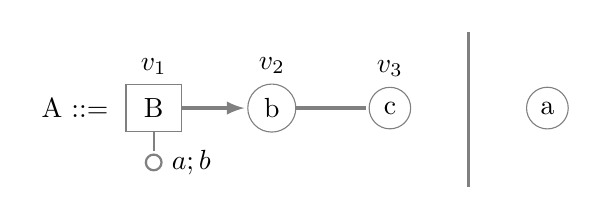
\begin{tikzpicture}[grammar]
			%The LHS
			\draw (0,0) node[lhs] (lhs) {A ::=};
			
			%The RHS graph
			\draw (1,0) node[nont, label=90:$v_1$] (v1) {B};
			\draw (2.5,0) node[t, label=90:$v_2$] (v2) {b};
			\draw (4,0) node[t, label=90:$v_3$] (v3) {c};
			
			\draw[edge] (v1) -- (v2);
			\draw[biedge] (v2) -- (v3);
			
			%The embedding
			\draw node[w, label=0:$a;b$] at (v1.south) (w-v1) {}
					[wedge] (v1) -- (w-v1);
			
			%The next rule separator
			\draw[pipe] (5,-1) -- (5,1);
			
			%The second RHS graph
			\draw (6,0) node[t] (u1) {a};
		\end{tikzpicture}
		
		Note that, we use squares for nodes labeled with non-terminal symbols, circles for nodes labeled with terminal symbols, position the respective label inside the shape and the (possibly omitted) identifier over it. To depict the embedding function, we place below the respective node a small circle labeled with the image of the embedding function for this node.
		
		%Examples (chains and activities)
		\begin{example}{Chains of a's and b's.}
			$GG = (\{S,A,B,a,b\}, \{a,b\}, P, S)$, where $P$ is\\
			
			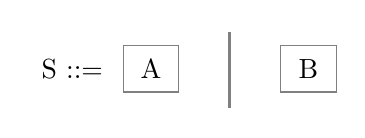
\begin{tikzpicture}[grammar]
				%The LHS
				\draw (0,0) node[lhs] (lhs) {S ::=};
				
				%The RHS graph
				\draw (1,0) node[nont] (v1) {A};
				
				%The next rule separator
				\draw[pipe] (2,-0.5) -- (2,0.5);
				
				%The second RHS graph
				\draw (3,0) node[nont] (v2) {B};
			\end{tikzpicture}
			
			\begin{tikzpicture}[grammar]
				%The LHS
				\draw (0,0) node[lhs] (lhs) {A ::=};
				
				%The RHS graph
				\draw (1,0) node[t] (v3) {a};
				\draw (2.5,0) node[nont] (v4) {B};
				
				\draw[edge] (v3) -- (v4);
				
				\draw node[w, label=0:$b$] at (v3.south) (w-v3) {}
					[wedge] (v1) -- (w-v3);
				
				%The next rule separator
				\draw[pipe] (3.5,-1) -- (3.5,0.5);
				
				%The second RHS graph
				\draw (4.5,0) node[t] (v5) {a};
			\end{tikzpicture}
			
			\begin{tikzpicture}[grammar]
				%The LHS
				\draw (0,0) node[lhs] (lhs) {B ::=};
				
				%The RHS graph
				\draw (1,0) node[t] (v6) {b};
				\draw (2.5,0) node[nont] (v7) {A};
				
				\draw[edge] (v3) -- (v4);
				
				\draw node[w, label=0:$a$] at (v6.south) (w-v6) {}
				[wedge] (v1) -- (w-v6);
				
				%The next rule separator
				\draw[pipe] (3.5,-1) -- (3.5,0.5);
				
				%The second RHS graph
				\draw (4.5,0) node[t] (v8) {b};
			\end{tikzpicture}
		\end{example}
		
		\begin{example}{Activity diagrams.}
			$GG = (\{S,A,F,D,L,a,c,e,if\}, \{a,c,e,if\}, P, S)$, where $P$ is\\
			
			\begin{tikzpicture}[grammar]
				%The LHS
				\draw (0,0) node[lhs] (lhs) {S ::=};
				
				%The RHS graph
				\draw (1,0) node[nont] (v1) {A};
				
				%The next rule separator
				\draw[pipe] (2,-0.5) -- (2,0.5);
				
				%The second RHS graph
				\draw (3,0) node[g] (v2) {$\emptyGraph$};
			\end{tikzpicture}
			
			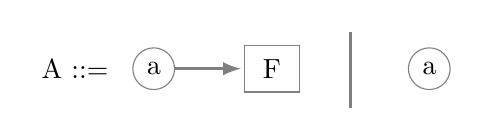
\begin{tikzpicture}[grammar]
				%The LHS
				\draw (0,0) node[lhs] (lhs) {A ::=};
				
				%The RHS graph
				\draw (1,0) node[t] (v1) {a};
				\draw (2.5,0) node[nont] (v2) {F};
				
				\draw[edge] (v1) -- (v2);
				
				%The next rule separator
				\draw[pipe] (3.5,-0.5) -- (3.5,0.5);
				
				%The second RHS graph
				\draw (4.5,0) node[t] (v3) {a};
			\end{tikzpicture}
			
			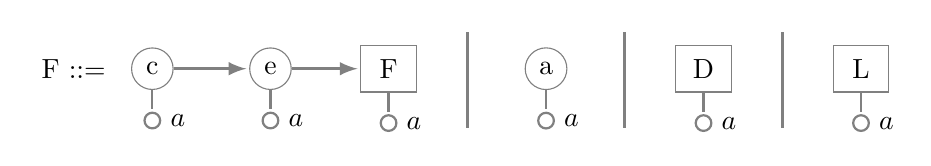
\begin{tikzpicture}[grammar]
				%The LHS
				\draw (0,0) node[lhs] (lhs) {F ::=};
				
				%The RHS graph
				\draw (1,0) node[t] (v1) {c};
				\draw (2.5,0) node[t] (v2) {e};
				\draw (4,0) node[nont] (v3) {F};
				
				\draw[edge] (v1) -- (v2);
				\draw[edge] (v2) -- (v3);
				
				\draw node[w, label=0:$a$] at (v1.south) (w-v1) {}
					[wedge] (v1) -- (w-v1);
				\draw node[w, label=0:$a$] at (v2.south) (w-v2) {}
					[wedge] (v2) -- (w-v2);
				\draw node[w, label=0:$a$] at (v3.south) (w-v3) {}
					[wedge] (v3) -- (w-v3);
				
				%The next rule separator
				\draw[pipe] (5,-0.75) -- (5,0.5);
				
				%The second RHS graph
				\draw (6,0) node[t] (v4) {a};
				\draw node[w, label=0:$a$] at (v4.south) (w-v4) {}
					[wedge] (v4) -- (w-v4);
				
				%The next rule separator
				\draw[pipe] (7,-0.75) -- (7,0.5);
				
				%The second RHS graph
				\draw (8,0) node[nont] (v5) {D};
				\draw node[w, label=0:$a$] at (v5.south) (w-v5) {}
					[wedge] (v5) -- (w-v5);
				
				%The next rule separator
				\draw[pipe] (9,-0.75) -- (9,0.5);
				
				%The second RHS graph
				\draw (10,0) node[nont] (v6) {L};
				\draw node[w, label=0:$a$] at (v6.south) (w-v6) {}
					[wedge] (v6) -- (w-v6);
			\end{tikzpicture}
			
			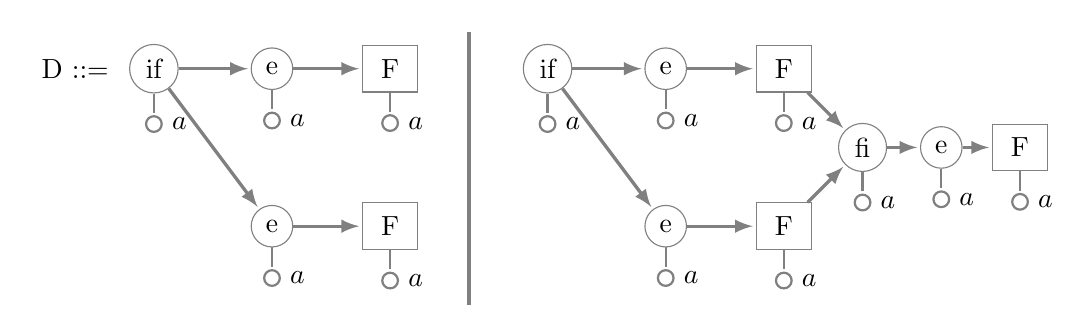
\begin{tikzpicture}[grammar]
				%The LHS
				\draw (0,0) node[lhs] (lhs) {D ::=};
				
				%The RHS graph
				\draw (1,0) node[t] (v1) {if};
				\draw (2.5,0) node[t] (v2) {e};
				\draw (4,0) node[nont] (v3) {F};
				\draw (2.5,-2) node[t] (v4) {e};
				\draw (4,-2) node[nont] (v5) {F};
				
				\draw[edge] (v1) -- (v2);
				\draw[edge] (v2) -- (v3);
				\draw[edge] (v1) -- (v4);
				\draw[edge] (v4) -- (v5);
				
				\draw node[w, label=0:$a$] at (v1.south) (w-v1) {}
					[wedge] (v1) -- (w-v1);
				\draw node[w, label=0:$a$] at (v2.south) (w-v2) {}
					[wedge] (v2) -- (w-v2);
				\draw node[w, label=0:$a$] at (v3.south) (w-v3) {}
					[wedge] (v3) -- (w-v3);
				\draw node[w, label=0:$a$] at (v4.south) (w-v4) {}
					[wedge] (v4) -- (w-v4);
				\draw node[w, label=0:$a$] at (v5.south) (w-v5) {}
					[wedge] (v5) -- (w-v5);
				
				%The next rule separator
				\draw[pipe] (5,-3) -- (5,0.5);
				
				%The second RHS graph
				\draw (6,0) node[t] (v6) {if};
				\draw (7.5,0) node[t] (v7) {e};
				\draw (9,0) node[nont] (v8) {F};
				\draw (7.5,-2) node[t] (v9) {e};
				\draw (9,-2) node[nont] (v10) {F};
				\draw (10,-1) node[t] (v11) {fi};
				\draw (11,-1) node[t] (v12) {e};
				\draw (12,-1) node[nont] (v13) {F};
				
				
				\draw[edge] (v6) -- (v7);
				\draw[edge] (v7) -- (v8);
				\draw[edge] (v6) -- (v9);
				\draw[edge] (v9) -- (v10);
				\draw[edge] (v10) -- (v11);
				\draw[edge] (v8) -- (v11);
				\draw[edge] (v11) -- (v12);
				\draw[edge] (v12) -- (v13);
				
				\draw node[w, label=0:$a$] at (v6.south) (w-v6) {}
					[wedge] (v6) -- (w-v6);
				\draw node[w, label=0:$a$] at (v7.south) (w-v7) {}
					[wedge] (v7) -- (w-v7);
				\draw node[w, label=0:$a$] at (v8.south) (w-v8) {}
					[wedge] (v8) -- (w-v8);
				\draw node[w, label=0:$a$] at (v9.south) (w-v9) {}
					[wedge] (v9) -- (w-v9);
				\draw node[w, label=0:$a$] at (v10.south) (w-v10) {}
					[wedge] (v10) -- (w-v10);
				\draw node[w, label=0:$a$] at (v11.south) (w-v11) {}
					[wedge] (v11) -- (w-v11);
				\draw node[w, label=0:$a$] at (v12.south) (w-v12) {}
					[wedge] (v12) -- (w-v12);
				\draw node[w, label=0:$a$] at (v13.south) (w-v13) {}
					[wedge] (v13) -- (w-v13);
			\end{tikzpicture}
			
			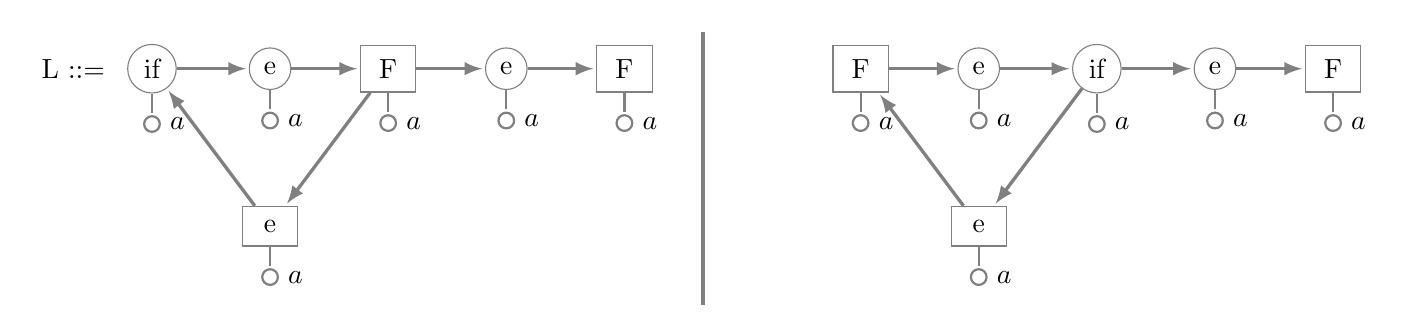
\begin{tikzpicture}[grammar]
				%The LHS
				\draw (0,0) node[lhs] (lhs) {L ::=};
				
				%The RHS graph
				\draw (1,0) node[t] (v1) {if};
				\draw (2.5,0) node[t] (v2) {e};
				\draw (4,0) node[nont] (v3) {F};
				\draw (5.5,0) node[t] (v4) {e};
				\draw (7,0) node[nont] (v5) {F};
				\draw (2.5,-2) node[nont] (v6) {e};
				
				\draw[edge] (v1) -- (v2);
				\draw[edge] (v2) -- (v3);
				\draw[edge] (v3) -- (v4);
				\draw[edge] (v4) -- (v5);
				\draw[edge] (v3) -- (v6);
				\draw[edge] (v6) -- (v1);
				
				\draw node[w, label=0:$a$] at (v1.south) (w-v1) {}
					[wedge] (v1) -- (w-v1);
				\draw node[w, label=0:$a$] at (v2.south) (w-v2) {}
					[wedge] (v2) -- (w-v2);
				\draw node[w, label=0:$a$] at (v3.south) (w-v3) {}
					[wedge] (v3) -- (w-v3);
				\draw node[w, label=0:$a$] at (v4.south) (w-v4) {}
					[wedge] (v4) -- (w-v4);
				\draw node[w, label=0:$a$] at (v5.south) (w-v5) {}
					[wedge] (v5) -- (w-v5);
				\draw node[w, label=0:$a$] at (v6.south) (w-v6) {}
					[wedge] (v6) -- (w-v6);
				
				%The next rule separator
				\draw[pipe] (8,-3) -- (8,0.5);
				
				%The second RHS graph
				\draw (10,0) node[nont] (v7) {F};
				\draw (11.5,0) node[t] (v8) {e};
				\draw (13,0) node[t] (v9) {if};
				\draw (14.5,0) node[t] (v10) {e};
				\draw (16,0) node[nont] (v11) {F};
				\draw (11.5,-2) node[nont] (v12) {e};
				
				\draw[edge] (v7) -- (v8);
				\draw[edge] (v8) -- (v9);
				\draw[edge] (v9) -- (v10);
				\draw[edge] (v10) -- (v11);
				\draw[edge] (v9) -- (v12);
				\draw[edge] (v12) -- (v7);
				
				\draw node[w, label=0:$a$] at (v7.south) (w-v7) {}
					[wedge] (v7) -- (w-v7);
				\draw node[w, label=0:$a$] at (v8.south) (w-v8) {}
					[wedge] (v8) -- (w-v8);
				\draw node[w, label=0:$a$] at (v9.south) (w-v9) {}
					[wedge] (v9) -- (w-v9);
				\draw node[w, label=0:$a$] at (v10.south) (w-v10) {}
					[wedge] (v10) -- (w-v10);
				\draw node[w, label=0:$a$] at (v11.south) (w-v11) {}
					[wedge] (v11) -- (w-v11);
				\draw node[w, label=0:$a$] at (v12.south) (w-v12) {}
					[wedge] (v12) -- (w-v12);
			\end{tikzpicture}
		\end{example}
		
		%Semantics
		The semantics of a B-NLC grammar is presented in the following. 
		
		\begin{definition}
			Let $G$ be a graph over $\Sigma$, $G$ is derived into $H$ with rule $r$ and vertex $v$, we write $G \deriv{r}{v} H$ and call it a derivation step, if and only if,
			\begin{align*}
				\exists r & = A \to R,w \in P \. \exists v \in V_G \.\\
				\phi_G(v) & = A \\
				V_H & = V_G \setminus \{v\} \cup V_R \\
				E_H & = E_G \setminus (\{(v,u) \st u \in V_G\} \cup \{(u,v) \st u \in V_G\}) \\
					& \cup E_R \\
					& \cup \{(u,t) \st (u,v) \in E_G \land \phi_G(u) \in w(t) \} \\
					& \cup \{(t,u) \st (v,u) \in E_G \land \phi_G(u) \in w(t) \} \\
				\phi_H & = (\phi_G \setminus \{(v,x)\}) \cup \phi_R
			\end{align*}
			Note that, without loss of generalization, we suppose that $V_G \cap V_R = \emptyset$, that is, the vertex sets are disjoint.
			Moreover, we denote with $\derivtr{}{}$ the transitive reflexive closure of $\deriv{}{}$.
		\end{definition}
		
		\begin{definition}
			A derivation $D$ is a sequence of derivation steps and is written as
			\[ 
				D = (G_0 \deriv{r_0}{v_0} G_1 \deriv{r_1}{v_1} G_2 \deriv{r_2}{v_2} \dots \deriv{r_{n-1}}{v_{n-1}} G_n)
			\]
		\end{definition}
		
		\begin{definition}
			The language $L(GG)$ generated by the graph grammar $GG = (\Sigma, \Delta, P, S)$ is 
			\[ L(GG) = \{G \st S \derivtr{}{} G \land \forall v \in V_G\. \phi_G(v) \in \Delta\}
			\]
		\end{definition}
		
		\begin{theorem}
			\label{thm:DerivationExistence}
			For every $G \in L(GG)$, there is at least one finite derivation
			\[ S \deriv{r_0}{v_0} H_1 \deriv{r_1}{v_1} H_2 \deriv{r_2}{v_2} \dots \deriv{r_{n-1}}{v_{n-1}} H_n \isomorph G
			\]
		\end{theorem}
		
		\begin{proof}
			...
		\end{proof}
		
		\begin{remark}
			It is not guaranteed that the derivation from Theorem \ref{thm:DerivationExistence} is unique. In the case that there are more than one derivation for a graph, we say that the grammar is ambiguous. Nevertheless, the grammar's ambiguity does not compromise the correctness of our algorithms presented in the following.
		\end{remark}
		
		%Parsing Algorithm
		Given a certain B-NLC graph grammar $GG$ and a graph $G$, we are interested in the problem of deciding if $G \in L(GG)$. This is sometimes called the \textit{membership} problem and can be solved through a recognizer algorithm that always finishes answering yes if and only if $G \in L(GG)$ and no otherwise. A slight extension of this problem is the \textit{parsing} problem, which consists of deciding if $G \in L(GG)$ and finding a derivation $S \derivtr{}{} G' \isomorph G$.
		
		The Algorithm \ref{alg:parse} is a correct (complete and consistent) parsing algorithm for any B-NLC graph grammar that runs in polynomial time and logarithmic space complexity. It has been taken from \cite{Rozenberg1986} and works in a bottom-up CYK-like (Cocke-Young-Kassami) manner.
		%TODO: Not sure about the logarithmic space complexity here
		
		%TODO: Preliminaries: V(R), Z(R)
		%TODO: Construct the derivation
		%TODO: Check that all symbols are in \Delta
		\begin{algorithm}[!h]
			\caption{Parsing Algorithm for B-NLC Graph Grammars}
			\begin{algorithmic}[!ht]
				\Function{$parse$}{$GG=(\Sigma, \Delta, P, S), G=(V_G,E_G,\phi_G)$}{$:Derivation$}
					\State $bup \gets \{(\phi_G(x),x) \st x \in V_G\}$
					\State $R_s \gets 2^{bup}$
					\Repeat
						\State $R \gets \text{any } \{r \in R_s \st V(r) \text{ is disjoint} \}$
						\State $T \gets T \cup \{R\}$
						\ForAll{$d \in \Sigma$}
							\If{$Z(\{(d,V(R))\}) \deriv{}{} Z(R)$}
								\State $bup \gets bup \cup \{(d,V(R))\}$
								\State $R_s \gets 2^{bup} \setminus T$
							\EndIf
						\EndFor
					\Until{$R_s \neq \emptyset$}
					\State \Return {$(S, V_G) \in bup \? true : false$}
				\EndFunction 
			\end{algorithmic}
			\label{alg:parse}
		\end{algorithm}
		%
		%Example
		%TODO: Give an example of an algorithm run
	\end{section}
	
	\begin{section}{Boundary Node-label Controlled Triple Graph Grammar}
		%Syntax
		In the following, based on the definitions of B-NLC graph grammar, we define the extension of the standard TGG \citep{schurr1994specification} specification, the B-NLC TGG.
		
		\begin{definition}
			A triple graph $TG = G_s \ms{m_s} G_c \mt{m_t} G_t$ over $\Sigma$ consists of three graphs $G_s$, $G_c$, $G_t$ over $\Sigma$, respectively, the source, correspondence and target graphs, together with two total morphisms $m_s: G_c \to G_s$ and $m_t: G_c \to G_t$. We denote the set of all triple graphs over $\Sigma$ as $\alltgraphs{\Sigma}$.
		\end{definition}
		
		\begin{definition}
			A $\Gamma\text{-boundary}$ triple graph $TG = G_s \ms{} G_c \mt{} G_t$ is such that $G_s$, $G_c$ and $G_t$ are $\Gamma\text{-boundary}$ graphs.
		\end{definition}		
		
		\begin{definition}
			A NLC triple graph grammar $TGG = (\Sigma, \Delta \subset \Sigma, P, S)$ consists of a finite set of symbols $\Sigma$, a set of terminal symbols $\Delta$ (define $\Gamma := \Sigma \setminus \Delta$), a set of production rules $P$ of the form $(A,B,C) \to TG,w_s,w_t$ with $A,B,C \in \Gamma$, $TG \in \alltgraphs{\Sigma}$ and two embedding functions $w_s: V_{G_s} \to 2^\Sigma$ and $w_t: V_{G_t} \to 2^\Sigma$.
		\end{definition}
		
		\begin{definition}
			A B-NLC TGG is a NLC TGG where for all rules $(A,B,C) \to TG,w_s,w_t \in P$, $TG$ is a boundary triple graph.
		\end{definition}
		
		%Example
		%TODO: Present the concrete syntax
		\begin{example}{Class Diagram to Java}
			$TGG = (\{S,C,A,I,m,p,k,a,prg,pck,cls,imp,att\}, \{m,p,k,a,prg,pck,$ $cls,imp,att,m_p,p_p,k_c,a_i,a_a,b_a\}, P, S)\}$, where $P$ is
			%TODO: Write the embedding in
			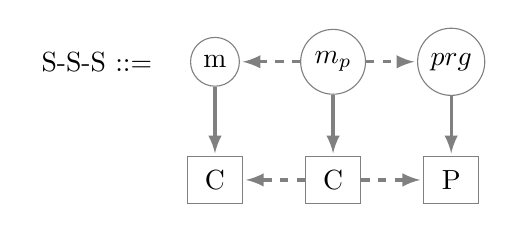
\begin{tikzpicture}[grammar]
				%The LHS
				\draw (-0.5,0) node[lhs] (lhs) {S-S-S ::=};
				
				%The RHS graph
				\draw (1,0) node[t] (s1) {m};
				\draw (2.5,0) node[t] (c1) {$m_p$};
				\draw (4,0) node[t] (t1) {$prg$};
				\draw (1,-1.5) node[nont] (s2) {C};
				\draw (2.5,-1.5) node[nont] (c2) {C};
				\draw (4,-1.5) node[nont] (t2) {P};
				
				\draw[edge] (s1) -- (s2);
				\draw[edge] (c1) -- (c2);
				\draw[edge] (t1) -- (t2);
				
				\draw[morph] (c1) -- (s1);
				\draw[morph] (c1) -- (t1);
				\draw[morph] (c2) -- (s2);
				\draw[morph] (c2) -- (t2);
			\end{tikzpicture}
			\\
			
			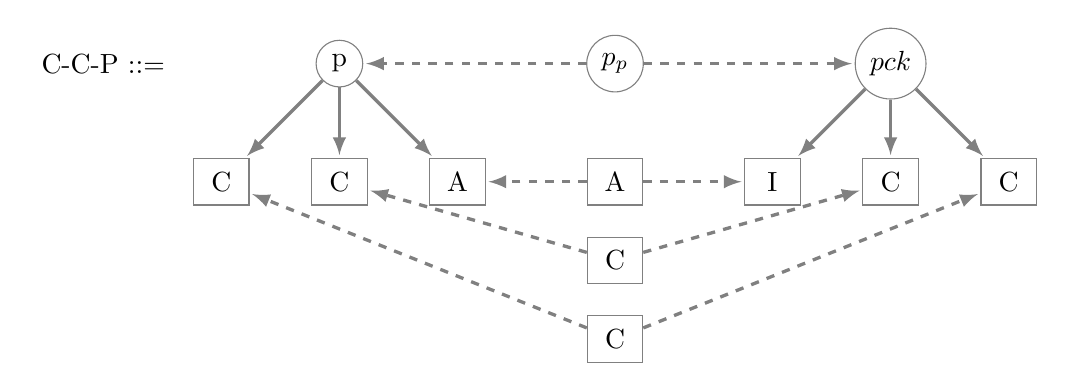
\begin{tikzpicture}[grammar]
				%The LHS
				\draw (-0,0) node[lhs] (lhs) {C-C-P ::=};
				
				%The RHS graph
				\draw (3,0) node[t] (s1) {p};
				\draw (1.5,-1.5) node[nont] (s2) {C};
				\draw (3,-1.5) node[nont] (s3) {C};
				\draw (4.5,-1.5) node[nont] (s4) {A};
				
				\draw (6.5,0) node[t] (c1) {$p_p$};
				\draw (6.5,-1.5) node[nont] (c2) {A};
				\draw (6.5,-2.5) node[nont] (c3) {C};
				\draw (6.5,-3.5) node[nont] (c4) {C};
				
				\draw (10,0) node[t] (t1) {$pck$};
				\draw (8.5,-1.5) node[nont] (t2) {I};
				\draw (10,-1.5) node[nont] (t3) {C};
				\draw (11.5,-1.5) node[nont] (t4) {C};
				
				\draw[edge] (s1) -- (s2);
				\draw[edge] (s1) -- (s3);
				\draw[edge] (s1) -- (s4);
				
				\draw[edge] (t1) -- (t2);
				\draw[edge] (t1) -- (t3);
				\draw[edge] (t1) -- (t4);
				
				\draw[morph] (c1) -- (s1);
				\draw[morph] (c1) -- (t1);
				\draw[morph] (c2) -- (s4);
				\draw[morph] (c2) -- (t2);
				\draw[morph] (c3) -- (s3);
				\draw[morph] (c3) -- (t3);
				\draw[morph] (c4) -- (s2);
				\draw[morph] (c4) -- (t4);
			\end{tikzpicture}
			\\
			
			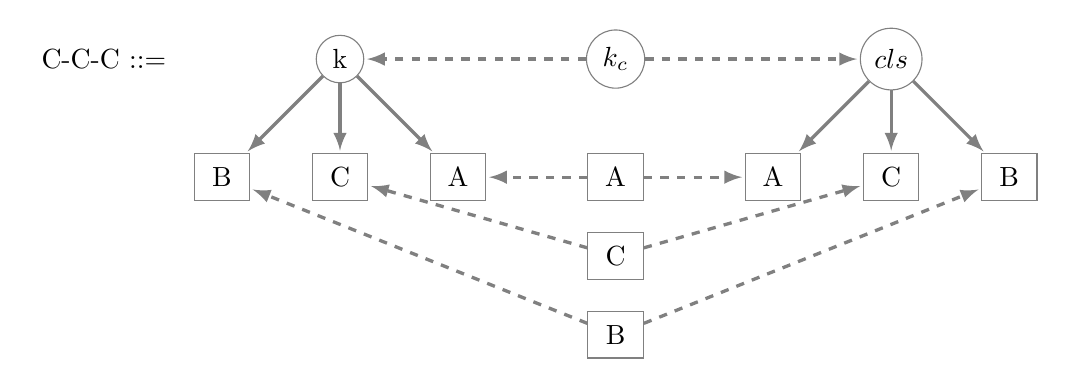
\begin{tikzpicture}[grammar]
				%The LHS
				\draw (-0,0) node[lhs] (lhs) {C-C-C ::=};
				
				%The RHS graph
				\draw (3,0) node[t] (s1) {k};
				\draw (1.5,-1.5) node[nont] (s2) {B};
				\draw (3,-1.5) node[nont] (s3) {C};
				\draw (4.5,-1.5) node[nont] (s4) {A};
				
				\draw (6.5,0) node[t] (c1) {$k_c$};
				\draw (6.5,-1.5) node[nont] (c2) {A};
				\draw (6.5,-2.5) node[nont] (c3) {C};
				\draw (6.5,-3.5) node[nont] (c4) {B};
				
				\draw (10,0) node[t] (t1) {$cls$};
				\draw (8.5,-1.5) node[nont] (t2) {A};
				\draw (10,-1.5) node[nont] (t3) {C};
				\draw (11.5,-1.5) node[nont] (t4) {B};
				
				\draw[edge] (s1) -- (s2);
				\draw[edge] (s1) -- (s3);
				\draw[edge] (s1) -- (s4);
				
				\draw[edge] (t1) -- (t2);
				\draw[edge] (t1) -- (t3);
				\draw[edge] (t1) -- (t4);
				
				\draw[morph] (c1) -- (s1);
				\draw[morph] (c1) -- (t1);
				\draw[morph] (c2) -- (s4);
				\draw[morph] (c2) -- (t2);
				\draw[morph] (c3) -- (s3);
				\draw[morph] (c3) -- (t3);
				\draw[morph] (c4) -- (s2);
				\draw[morph] (c4) -- (t4);
			\end{tikzpicture}
			\\
			
			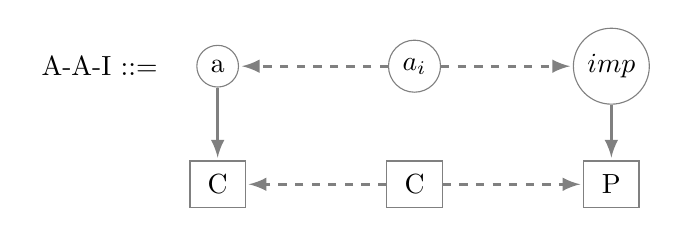
\begin{tikzpicture}[grammar]
				%The LHS
				\draw (-0,0) node[lhs] (lhs) {A-A-I ::=};
				
				%The RHS graph
				\draw (1.5,0) node[t] (s1) {a};
				\draw (1.5,-1.5) node[nont] (s2) {C};
				
				\draw (4,0) node[t] (c1) {$a_i$};
				\draw (4,-1.5) node[nont] (c2) {C};
				
				\draw (6.5,0) node[t] (t1) {$imp$};
				\draw (6.5,-1.5) node[nont] (t2) {P};
				
				\draw[edge] (s1) -- (s2);
				
				\draw[edge] (t1) -- (t2);
				
				\draw[morph] (c1) -- (s1);
				\draw[morph] (c1) -- (t1);
				\draw[morph] (c2) -- (s2);
				\draw[morph] (c2) -- (t2);
			\end{tikzpicture}
			\\
			
			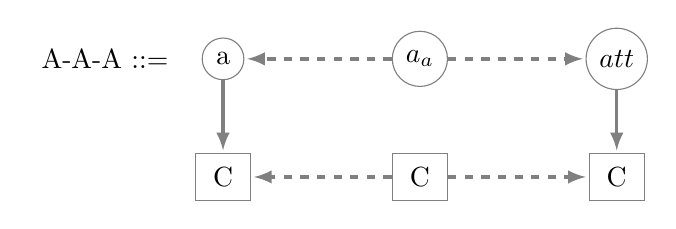
\begin{tikzpicture}[grammar]
				%The LHS
				\draw (-0,0) node[lhs] (lhs) {A-A-A ::=};
				
				%The RHS graph
				\draw (1.5,0) node[t] (s1) {a};
				\draw (1.5,-1.5) node[nont] (s2) {C};
				
				\draw (4,0) node[t] (c1) {$a_a$};
				\draw (4,-1.5) node[nont] (c2) {C};
				
				\draw (6.5,0) node[t] (t1) {$att$};
				\draw (6.5,-1.5) node[nont] (t2) {C};
				
				\draw[edge] (s1) -- (s2);
				\draw[edge] (t1) -- (t2);
				
				\draw[morph] (c1) -- (s1);
				\draw[morph] (c1) -- (t1);
				\draw[morph] (c2) -- (s2);
				\draw[morph] (c2) -- (t2);
			\end{tikzpicture}
			\\
			
			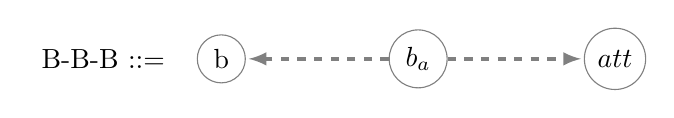
\begin{tikzpicture}[grammar]
				%The LHS
				\draw (-0,0) node[lhs] (lhs) {B-B-B ::=};
				
				%The RHS graph
				\draw (1.5,0) node[t] (s1) {b};
				
				\draw (4,0) node[t] (c1) {$b_a$};
				
				\draw (6.5,0) node[t] (t1) {$att$};
				
				\draw[morph] (c1) -- (s1);
				\draw[morph] (c1) -- (t1);
			\end{tikzpicture}
		\end{example}
		
		%Semantics
		%TODO: Write about the semantics. Should be very analogous to the simple graph grammar
		
		%Transformation Algorithm
		A consensus between the researchers of TGG is that the formalism aims at describing a consistency relation between two metamodels. In order to use it for transformation, it is necessary to operationalize it. In our case, the operationalization of the B-NLC TGG consists of deriving source and target rules from the production rules, which allows us to parse our input model and find a respective derivation using the Algorithm \ref{alg:parse}, to, then, generate the consistent triple graph containing the input and output models.
		
		\begin{definition}
			The derivation of source (target) rules from a B-NLC triple graph grammar $TGG=(\Sigma, \Delta, P, S)$ is done by creating a new B-NLC graph grammar $GG = (\Sigma, \Delta, \overline{P}, S)$, where for all rule $r_i = (A,B,C) \to G_s \ms{} G_c \mt{} G_t,w_s,w_t \in P$, there is a correspondent rule $\overline{r_i} = A \to G_s, w_s$ ($\overline{r_i} = C \to G_t, w_t$) in $\overline{P}$ and there is no other rule in $\overline{P}$.
		\end{definition}
		
		The Algorithm \ref{alg:fwd-transform} transforms a source graph into a target graph according to a triple graph grammar.
		\begin{algorithm}[!h]
			\caption{Forward Transformation Algorithm for B-NLC Triple Graph Grammars}
			\begin{algorithmic}[!ht]
				\Function{$fwd-transform$}{$TGG=(\Sigma, \Delta, P, S), G=(V_G,E_G,\phi_G)$}{$:Graph$}
					\State $GG \gets \text{source rules derived from }TGG$
					\State $D \gets parse(GG,G)$
					\If{$D \textbf{ is } S \deriv{\overline{r_0}}{v_0} H_0 \deriv{\overline{r_1}}{v_1} \dots \deriv{\overline{r_n}}{v_n} H_n \isomorph G$}
						\State $\textbf{let } S \ms{} S \mt{} S \deriv{r_0}{v_0} TG_0 \deriv{r_1}{v_1} \dots \deriv{r_n}{v_n} TG_n = G_s \ms{} G_c \mt{} G_t$
						\State \Return {$G_t$}
					\Else
						\State \Return {$fail$}
					\EndIf
				\EndFunction 
			\end{algorithmic}
			\label{alg:fwd-transform}
		\end{algorithm}
		
		%Incremental and Synchhronization
		%TODO: discourse about incremental transformation and synchronization
	\end{section}
	
	\begin{section}{Evaluation}
	\end{section}
	
	\bibliographystyle{authordate1}
	\bibliography{bibliography}
\end{homeworkProblem}

\end{document}

